% 05-Resultados_Presentacion_Tesis.tex
% Diapositivas de la sección Resultados

\section{Resultados}

\begin{frame}
\frametitle{Resumen de Resultados}
\begin{itemize}
    \item \textbf{Modelo ResNet50}: AUC-ROC Global-15 = 0.852
    \begin{itemize}
        \item Supera a CheXNet (0.841) y otros métodos del estado del arte
        \item COVID-19: AUC-ROC = 0.991, F1-Score = 0.799
    \end{itemize}
    \item \textbf{Modelo ViT}: AUC-ROC Global-15 = 0.791
    \begin{itemize}
        \item COVID-19: AUC-ROC = 0.982, F1-Score = 0.801
        \item Limitado por resolución de imagen (384x384)
    \end{itemize}
    \item \textbf{Comparación con radiólogos}: Los modelos superan a radiólogos en 6/15 patologías
\end{itemize}
\end{frame}

\begin{frame}
\frametitle{Comparación con el Estado del Arte}
\begin{table}[ht!]
    \centering
    \tiny
    \begin{tabular}{|l||c|c|c|c|c|c|c|l|}
        \hline
        \multicolumn{1}{|c||}{Patología}	&	\multicolumn{5}{c|}{\bf Modelos comparativos}    &\multicolumn{2}{c|}{\bf Propuestas} & 	\\
        \cline{2-9}
                        &	CRAL	&	DR-CNN	&	TSNC	& LgMeta & CheXNet	& CNN	    & ViT & 	Radiol.	\\
        \hline\hline
        Cardiomegaly	&	0.880	&	0.801	&	0.887	&	0.875	&\bf{0.923}	&	0.875	& 0.866 &	0.888	\\
        Emphysema	    &	0.908	&	0.773	&	0.930	&	0.895	&	0.937	&\bf{0.938}	& 0.866 &   0.911	\\
        Effusion	    &	0.829	&	0.797	&	0.831	&	0.822	&\bf{0.864}	&	0.850	& 0.791 &   0.900*	\\
        Hernia	        &	0.917	&	0.748	&	0.921	&\bf{0.937}	&	0.916	&	0.855	& 0.843 &   0.985*	\\
        Infiltration	&	0.702	&\bf{0.751}	&	0.703	&	0.694	&	0.734	&	0.740	& 0.621 &	0.734	\\
        Mass	        &	0.834	&	0.760	&	0.833	&	0.820	&\bf{0.868}	&	0.831	& 0.768 &	0.886*	\\
        Nodule	        &	0.773	&	0.741	&	0.798	&	0.747	&	0.780	&\bf{0.806}	& 0.704 &	0.899*	\\
        Atelectasis	    &	0.781	&	0.766	&	0.785	&	0.763	&\bf{0.809}	&	0.794	& 0.734 &	0.808	\\
        Pneumothorax	&	0.729	&	0.778	&	0.731	&	0.840	&	0.889	&\bf{0.906}	& 0.842 &	0.940*	\\
        Pleural-Thick.	&	0.778	&	0.759	&	0.782	&	0.763	&	0.806	&\bf{0.820}	& 0.765 &	0.779	\\
        Pneumonia	    &	0.857	&	0.800	&\bf{0.881}	&	0.731	&	0.768	&	0.863	& 0.738 &	0.823	\\
        Fibrosis	    &	0.830	&	0.765	&	0.833	&	0.816	&	0.805	&\bf{0.852}	& 0.810 &	0.897*	\\
        Edema	        &	0.850	&	0.820	&	0.849	&	0.846	&\bf{0.888}	&	0.879	& 0.828 &	0.910*	\\
        Consolidation	&	0.754	&	0.787	&	0.754	&	0.749	&\bf{0.790}	&	0.776	& 0.715 &	0.841*	\\
        \hline
        COVID-19	    &	---	    &	---	    &	---	    &	---	    &	---	    &\bf{0.991}	& 0.982 &	---	    \\
        Healthy	        &	---	    &	---	    &	---	    &	0.727	&	---	    &\bf{0.736}	& 0.705 &	---	    \\
        \hline\hline
        Global-14	    &	0.816	&	0.775	&	0.823	&	0.807	&	0.841	&\bf{0.842}	& 0.778 &	0.872*	\\
        Global-15	    &	---	    &	---	    &	---	    &	---	    &	---	    &\bf{0.852}	& 0.791 &	---	    \\
        \hline
    \end{tabular}
    \caption{Valores correspondientes a la métrica AUC-ROC para las 15 patologías y muestras saludables.}
    \label{table_roc_auc}
\end{table}
\end{frame}

\begin{frame}
\frametitle{Resultados por Patología - ResNet50 vs ViT}
\begin{table}[ht!]
    \centering
    \tiny
    \begin{tabular}{|l||c|c|c|c||c|c|c|c|}
        \hline
        {\bf Patología} & \multicolumn{4}{c||}{\bf ResNet50} & \multicolumn{4}{c|}{\bf ViT} \\
        \cline{2-9}
         & AUC-PR & AUC-ROC & F1-Score & Acc. & AUC-PR & AUC-ROC & F1-Score & Acc. \\
        \hline\hline
        Cardiomegaly    & 0.290 & 0.875 & 0.324 & 0.911 & 0.253 & 0.866 & 0.324 & 0.928 \\
        Emphysema       & 0.413 & 0.938 & 0.350 & 0.886 & 0.246 & 0.866 & 0.319 & 0.924 \\
        Effusion        & 0.494 & 0.850 & 0.527 & 0.807 & 0.401 & 0.791 & 0.434 & 0.807 \\
        Hernia          & 0.050 & 0.855 & 0.051 & 0.957 & 0.036 & 0.843 & 0.064 & 0.971 \\
        Infiltration    & 0.382 & 0.740 & 0.458 & 0.711 & 0.256 & 0.621 & 0.235 & 0.724 \\
        Mass            & 0.290 & 0.831 & 0.340 & 0.877 & 0.227 & 0.768 & 0.296 & 0.900 \\
        Nodule          & 0.249 & 0.806 & 0.299 & 0.876 & 0.157 & 0.704 & 0.209 & 0.908 \\
        Atelectasis     & 0.336 & 0.794 & 0.387 & 0.815 & 0.271 & 0.734 & 0.325 & 0.840 \\
        Pneumothorax    & 0.447 & 0.906 & 0.496 & 0.852 & 0.359 & 0.842 & 0.430 & 0.880 \\
        Pleural-Thick   & 0.157 & 0.820 & 0.217 & 0.852 & 0.125 & 0.765 & 0.197 & 0.881 \\
        Pneumonia       & 0.425 & 0.863 & 0.274 & 0.856 & 0.104 & 0.738 & 0.144 & 0.732 \\
        Fibrosis        & 0.106 & 0.852 & 0.154 & 0.910 & 0.070 & 0.810 & 0.134 & 0.932 \\
        Edema           & 0.187 & 0.879 & 0.193 & 0.788 & 0.120 & 0.828 & 0.180 & 0.877 \\
        Consolidation   & 0.150 & 0.776 & 0.234 & 0.754 & 0.118 & 0.715 & 0.171 & 0.836 \\
        \hline
        COVID-19        & 0.844 & 0.991 & 0.799 & 0.969 & 0.859 & 0.982 & 0.801 & 0.973 \\
        Healthy         & 0.691 & 0.736 & 0.496 & 0.712 & 0.634 & 0.705 & 0.537 & 0.703 \\
        \hline\hline
        Global-14       & 0.284 & 0.842 & 0.307 & 0.847 & 0.196 & 0.778 & 0.247 & 0.867 \\
        Global-15       & 0.321 & 0.852 & 0.340 & 0.855 & 0.240 & 0.791 & 0.284 & 0.874 \\
        \hline
    \end{tabular}
    \caption{Resumen del rendimiento de los modelos propuestos basados en \textit{ResNet50} y \textit{ViT} para cada patología.}
    \label{table:res-vit-model-covid}
\end{table}
\end{frame}

\begin{frame}
\frametitle{Curvas ROC - ResNet50}
\begin{figure}[ht!]
    \centering
    \includegraphics[width=0.5\textwidth]{../Chapters/4. ViT-Lung/images/ROC_AUC.pdf}
    \caption{Curvas ROC del modelo ResNet50 para todas las patologías.}
\end{figure}
\end{frame}

\begin{frame}
\frametitle{Curvas ROC - ViT}
\begin{figure}[ht!]
    \centering
    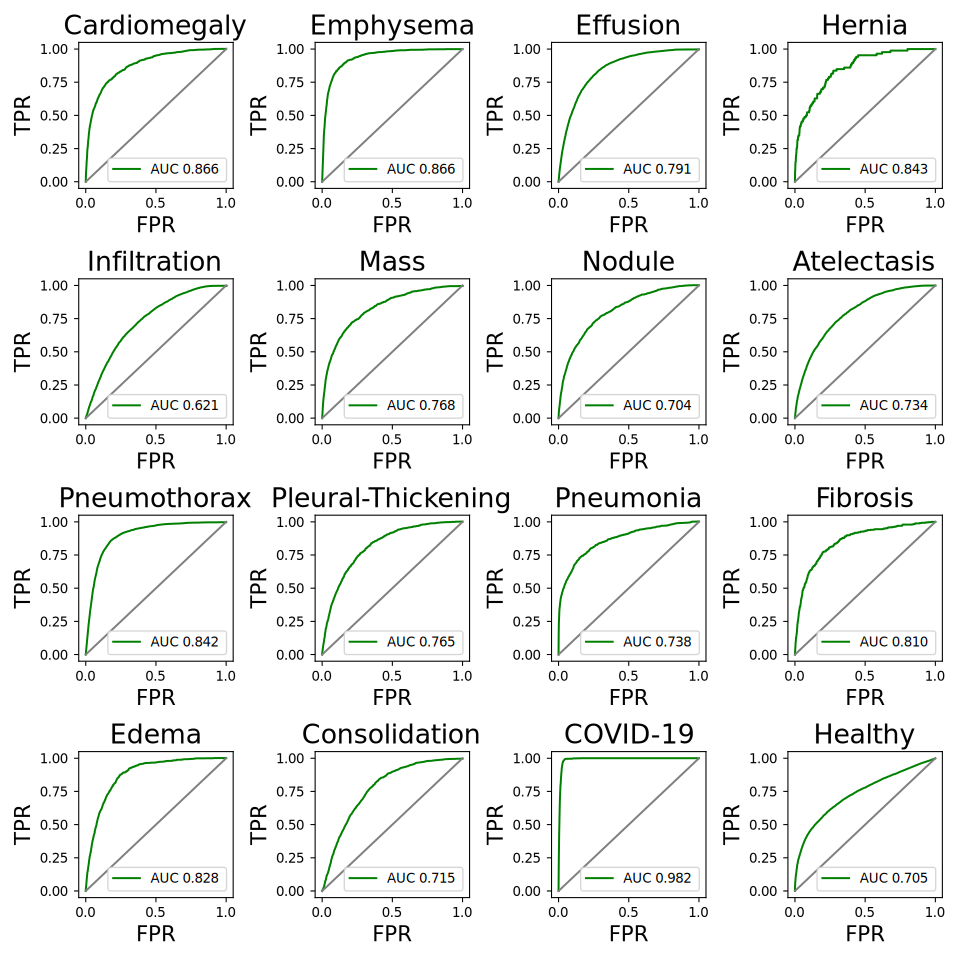
\includegraphics[width=0.5\textwidth]{../Chapters/4. ViT-Lung/images/ROC_AUC_ViT.pdf}
    \caption{Curvas ROC del modelo ViT. Mantiene buen rendimiento a pesar de menor resolución.}
\end{figure}
\end{frame}

\begin{frame}
\frametitle{Visualización de Atención - GradCAM}
\begin{figure}[ht!]
    \centering
    \includegraphics[width=0.8\textwidth]{../Chapters/4. ViT-Lung/images/vlgrid.png}
    \caption{Ejemplos de visualización GradCAM: Cardiomegaly, Pneumonia, Mass y COVID-19. Las regiones rojas indican las áreas de mayor atención del modelo.}
\end{figure}
\end{frame}

\begin{frame}
\frametitle{Comparación con Radiólogos Humanos}
\begin{table}[ht!]
    \centering
    \tiny
    \begin{tabular}{|l||l|c|l|}
        \hline
                        &	Method	&	AUC-ROC	& Radiol.	\\
        \hline\hline
        Cardiomegaly	&	CheXNet	    & 0.923 &   0.888	\\
        Emphysema	    &	Proposal    & 0.938	&   0.911	\\
        Effusion	    &	CheXNet	    & 0.864 &   0.900*	\\
        Hernia	        &	LargeMeta   & 0.937	&   0.985*	\\
        Infiltration	&	DR-CNN	    & 0.751 &	0.734	\\
        Mass	        &	CheXNet	    & 0.868	&	0.886*	\\
        Nodule	        &	Proposal    & 0.806	&	0.899*	\\
        Atelectasis	    &	CheXNet	    & 0.809 &	0.808	\\
        Pneumothorax	&	Proposal    & 0.906 &	0.940*	\\
        Pleural-Thick.	&	Proposal    & 0.820	&	0.779	\\
        Pneumonia	    &	TSNC	    & 0.881 &	0.823	\\
        Fibrosis	    &	Proposal    & 0.852 &	0.897*	\\
        Edema	        &	CheXNet	    & 0.888 &	0.910*	\\
        Consolidation	&	CheXNet	    & 0.790 &	0.841*	\\
        COVID-19	    &	Proposal    & 0.991 &	------	\\
        \hline
    \end{tabular}
    %}
    \caption{Comparativo por patología de los modelos de deep learning con mejor rendimiento contra
             el rendimiento de los radiólogos humanos. Los radiólogos lideran en 8 de las 15
             patologías.}
    \label{table_dl_human}
\end{table}
\end{frame}

\begin{frame}
\frametitle{Extensión a Tuberculosis - Resultados}
\begin{itemize}
    \item \textbf{Clasificador binario para tuberculosis}
    \begin{itemize}
        \item F1-Score: 0.707
        \item Accuracy: 0.846
        \item Verdaderos positivos: 388/488 casos
    \end{itemize}
    \item \textbf{Análisis en modelo de 15 patologías}
    \begin{itemize}
        \item ResNet50: 480 casos detectados como COVID-19, 93 como neumonía
        \item ViT: 481 casos como COVID-19, 2 como neumonía
        \item Comportamiento esperado debido a similitudes radiológicas
    \end{itemize}
\end{itemize}
\end{frame}

\begin{frame}
\frametitle{Análisis de Limitaciones y Fortalezas}
\begin{columns}
\column{0.5\textwidth}
\textbf{ResNet50 - Fortalezas:}
\begin{itemize}
    \item Mayor resolución (1024x1024)
    \item Mejor rendimiento global
    \item Más épocas de entrenamiento
    \item Arquitectura probada
\end{itemize}

\column{0.5\textwidth}
\textbf{ViT - Fortalezas:}
\begin{itemize}
    \item Convergencia más rápida
    \item Menos épocas necesarias
    \item Atención global
    \item Arquitectura moderna
\end{itemize}

\textbf{Limitación principal:}
\begin{itemize}
    \item Consumo de memoria alto
    \item Resolución limitada (384x384)
\end{itemize}
\end{columns}
\end{frame}

% \begin{frame}
% \frametitle{Conclusiones de Resultados}
% \begin{itemize}
%     \item \textbf{Rendimiento excepcional}
%     \begin{itemize}
%         \item ResNet50 establece nuevo estándar (AUC-ROC Global-15: 0.852)
%         \item COVID-19: AUC-ROC de 0.991 (ResNet50) y 0.982 (ViT)
%     \end{itemize}
%     \item \textbf{Superación del estado del arte}
%     \begin{itemize}
%         \item Lidera en 5 patologías específicas
%         \item Supera a radiólogos en 6/15 patologías
%     \end{itemize}
%     \item \textbf{Versatilidad demostrada}
%     \begin{itemize}
%         \item Extensión exitosa a tuberculosis
%         \item Interpretabilidad clínica con GradCAM
%     \end{itemize}
%     \item \textbf{Impacto clínico potencial}
%     \begin{itemize}
%         \item Herramienta valiosa para apoyo diagnóstico
%         \item Capacidad de adaptación a nuevas patologías
%     \end{itemize}
% \end{itemize}
% \end{frame}
